% Latex template: https://github.com/mqTeXUsers/Macquarie-University-Beamer-Theme


\documentclass[aspectratio=169, 11pt]{beamer} % Aspect ratio
% https://tex.stackexchange.com/a/14339/5483 


\usetheme{macquarie}

\mode<presentation>           % Set options
{
  \usetheme{default}          % Set theme
  \usecolortheme{default}         % Set colors
  \usefonttheme{default}          % Set font theme
  \setbeamertemplate{caption}[numbered] % Set caption to be numbered
}


\setbeamertemplate{footline}{%
%\strut~\texttt{https://github.com/MQ-FOAR705/MQ-FOAR705-Week1}%
\hfill\insertframenumber~/~\inserttotalframenumber\strut~~~
}


\title{Strategic Approaches for Technologically enabled Research and Data Science} % Presentation title
\author{Brian Ballsun-Stanton}               % Presentation author
\institute{Faculty of Arts}         % Author affiliation
\date{12 August 2020}                 % Today's date  

%https://tex.stackexchange.com/questions/522541/beamer-biblatex-includeonlylecture-works-but-bibliography-global
  \addbibresource{references.bib}


\begin{document}



\maketitle

\begin{frame}{Introduction}
\textbf{Dr Brian Ballsun-Stanton -- Solutions Architect (Digital Humanities)}
\begin{multicols}{2}
\begin{itemize}
    \item PhD UNSW 2012 in the Philosophy of Data. 
    \item BS and MS at Rochester Institute of Technology in Information Technology.
    \item \$2,262,449 in Grants and Prizes
    \item 23 Projects across the faculty since 2017 including Philosophy, Security Studies, and Ancient History.
\end{itemize}
\end{multicols}

\begin{figure}

    \begin{subfigure}{.19\textwidth}
    \centering
    %\includegraphics[width=\linewidth]{figures/truck.jpg}
    \adjincludegraphics[width=\linewidth,height=\linewidth,trim={{.25\width} 0 {.25\width} 0},clip]{figures/truck.jpg}

    \caption{63 field data collection projects}
    \end{subfigure}%https://www.overleaf.com/project/5f27849a137f300001cd5264
    \hfill%
    \begin{subfigure}{.19\textwidth}

    
\includegraphics[width=\linewidth]{figures/onwork-screenshot.png}
    %\adjincludegraphics[width=\linewidth,trim={0 0 0 {.5\linewidth}},clip]{figures/onwork-screenshot.png}
    \caption{onwork.edu.au, indexing 2000 citations}
    \end{subfigure}%
    \hfill%
    \begin{subfigure}{.19\textwidth}
    \centering
    
\includegraphics[width=\linewidth]{figures/gac-screenshot.png}
    \caption{MQ's Partnership with Google Arts \& Culture. 15,820 views in July 2020 }
    \end{subfigure}
    \caption{Images from recent projects}
\end{figure}

\end{frame}

\begin{frame}{Outline of Talk}
  \tableofcontents
\end{frame}

%During the presentation, you will present to our eResearch and Data Science Steering Committee (which overlaps in part with the Selection Panel) and includes Associate Deans Research, the Directors of IT, Library, Research Integrity and others. 

%These are the main stakeholders of the role. Professor Amanda Barnier would like each candidate to speak for about 20 minutes and cover: 

    %(1) his or her view of the importance of eResearch and Data Science to modern research practices, 
    %(2) one or two examples of his or her own research illustrating these practices (whether research he or she has led or research he or she has supported others in conducting), and 
    %(3) how you can help Macquarie transform its research practices in this space.
\section{Technologically Enabled Research}

\begin{frame}{Technology, Data, Systems}

\textbf{Technology:} \begin{quote}
... technologies either as
\textbf{objects} (the stethoscope, the rifle), \textbf{practices} (disciplinary techniques), \textbf{knowledge} (medicine and penology), modes of \textbf{organization} (hospital, school, prison), or frequently,
by the \textbf{conglomeration} of these. \parencite{Lagdameo2019-sa}
\end{quote} 

\textbf{Data:}
\begin{quote}
Data as objective \textbf{measure}, Data as subjective \textbf{observation}, Data as encoded human \textbf{communication} \parencite{Ballsun-Stanton2012-nx}
\end{quote}

\textbf{System:}
\begin{quote}
According to the
cybernetician, \textbf{the purpose of a system is what it does.} This is a basic dictum. It stands for a bald fact, which makes a better starting point in seeking understanding than the familiar
attributions of good intentions... \parencite{Beer2002-tl}
\end{quote} 
\end{frame}

\begin{frame}{Ethical Considerations}

\textbf{Reduce the number of redundant studies because we don't have the data}
\begin{itemize}
    \item `As open as possible, as closed as necessary.' \parencite{European_Commission2016-ai}
    \item The replication crisis and our duties to future scholarship \parencite{Hochstrasser2020-mr,  National_Academies_of_Sciences_Engineering_and_Medicine2019-da, Reed2014-aa, Franco2014-oy}
    \end{itemize}

% \mbox{}\hfill\raisebox{-\height}[0pt][0pt]{\begin{figure}
\includegraphics[width=.25\linewidth]{figures/qld-breach.png}
% QLD Health breach article. \parencite{Bavas2019-xc}}
% }

%\vspace{5mm}
\begin{columns}[t]
\begin{column}{.35\textwidth}
\textbf{Reduce harm to participants, researchers, institutions}    
\begin{itemize}
    \item Automation
    \item NHMRC Compliance
    % \begin{itemize}
    %     \item Prevent harm to research subjects.
    %     \item Make sure data is robust and available to others in future.
    % \end{itemize}
    \item Reduce impact of breaches
    % \begin{itemize}
    %     \item Automate protections to lower workload
    %     \item Do not rely on a lack-of-laptops left in taxis
    % \end{itemize}
    
    
\end{itemize}
\vfill
\end{column}
\begin{column}{.3\textwidth}
\begin{figure}
    \centering
    \vspace{-8mm}
    
\includegraphics[width=\linewidth]{figures/qld-breach.png}
    \caption{QLD Health breach. \parencite{Bavas2019-xc}}
\end{figure}
\end{column}
\begin{column}{.3\textwidth}

\begin{figure}
    \centering
    \vspace{-8mm}
    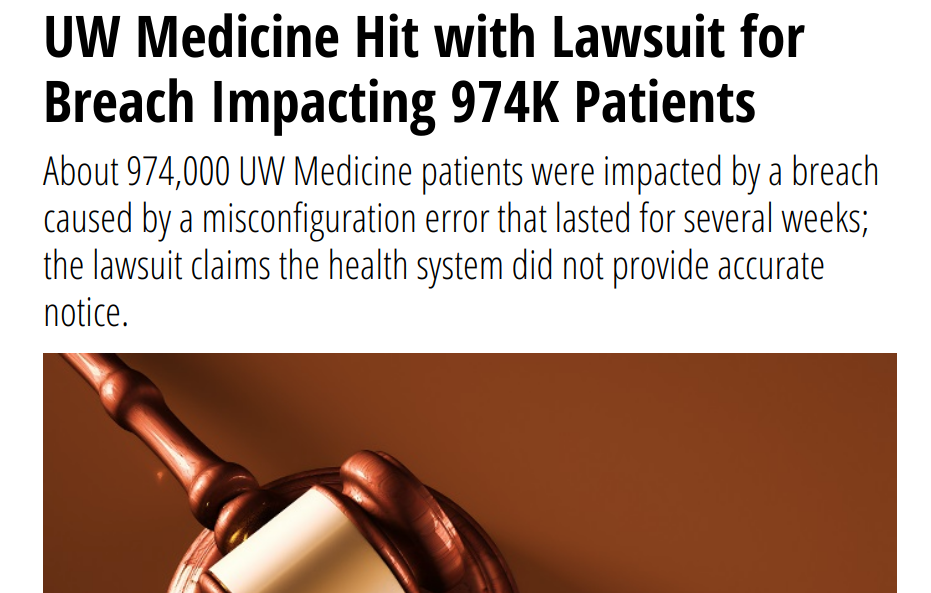
\includegraphics[width=\linewidth]{figures/uw.png}
     %\adjincludegraphics[width=\linewidth,trim={0 {.2\linewidth} 0 0},clip]{figures/uw.png}
    \caption{Consequences of drives left in a safe. \parencite{Davis2020-jr}}
\end{figure}

\end{column}
\end{columns}



\end{frame}


\setbeamertemplate{footline}{%
%\strut~\texttt{https://github.com/MQ-FOAR705/MQ-FOAR705-Week1}%
Photo by Franck V on Unplash, https://unsplash.com/photos/U3sOwViXhkY\hfill\insertframenumber~/~\inserttotalframenumber\strut~~~
}

{\usebackgroundtemplate{%
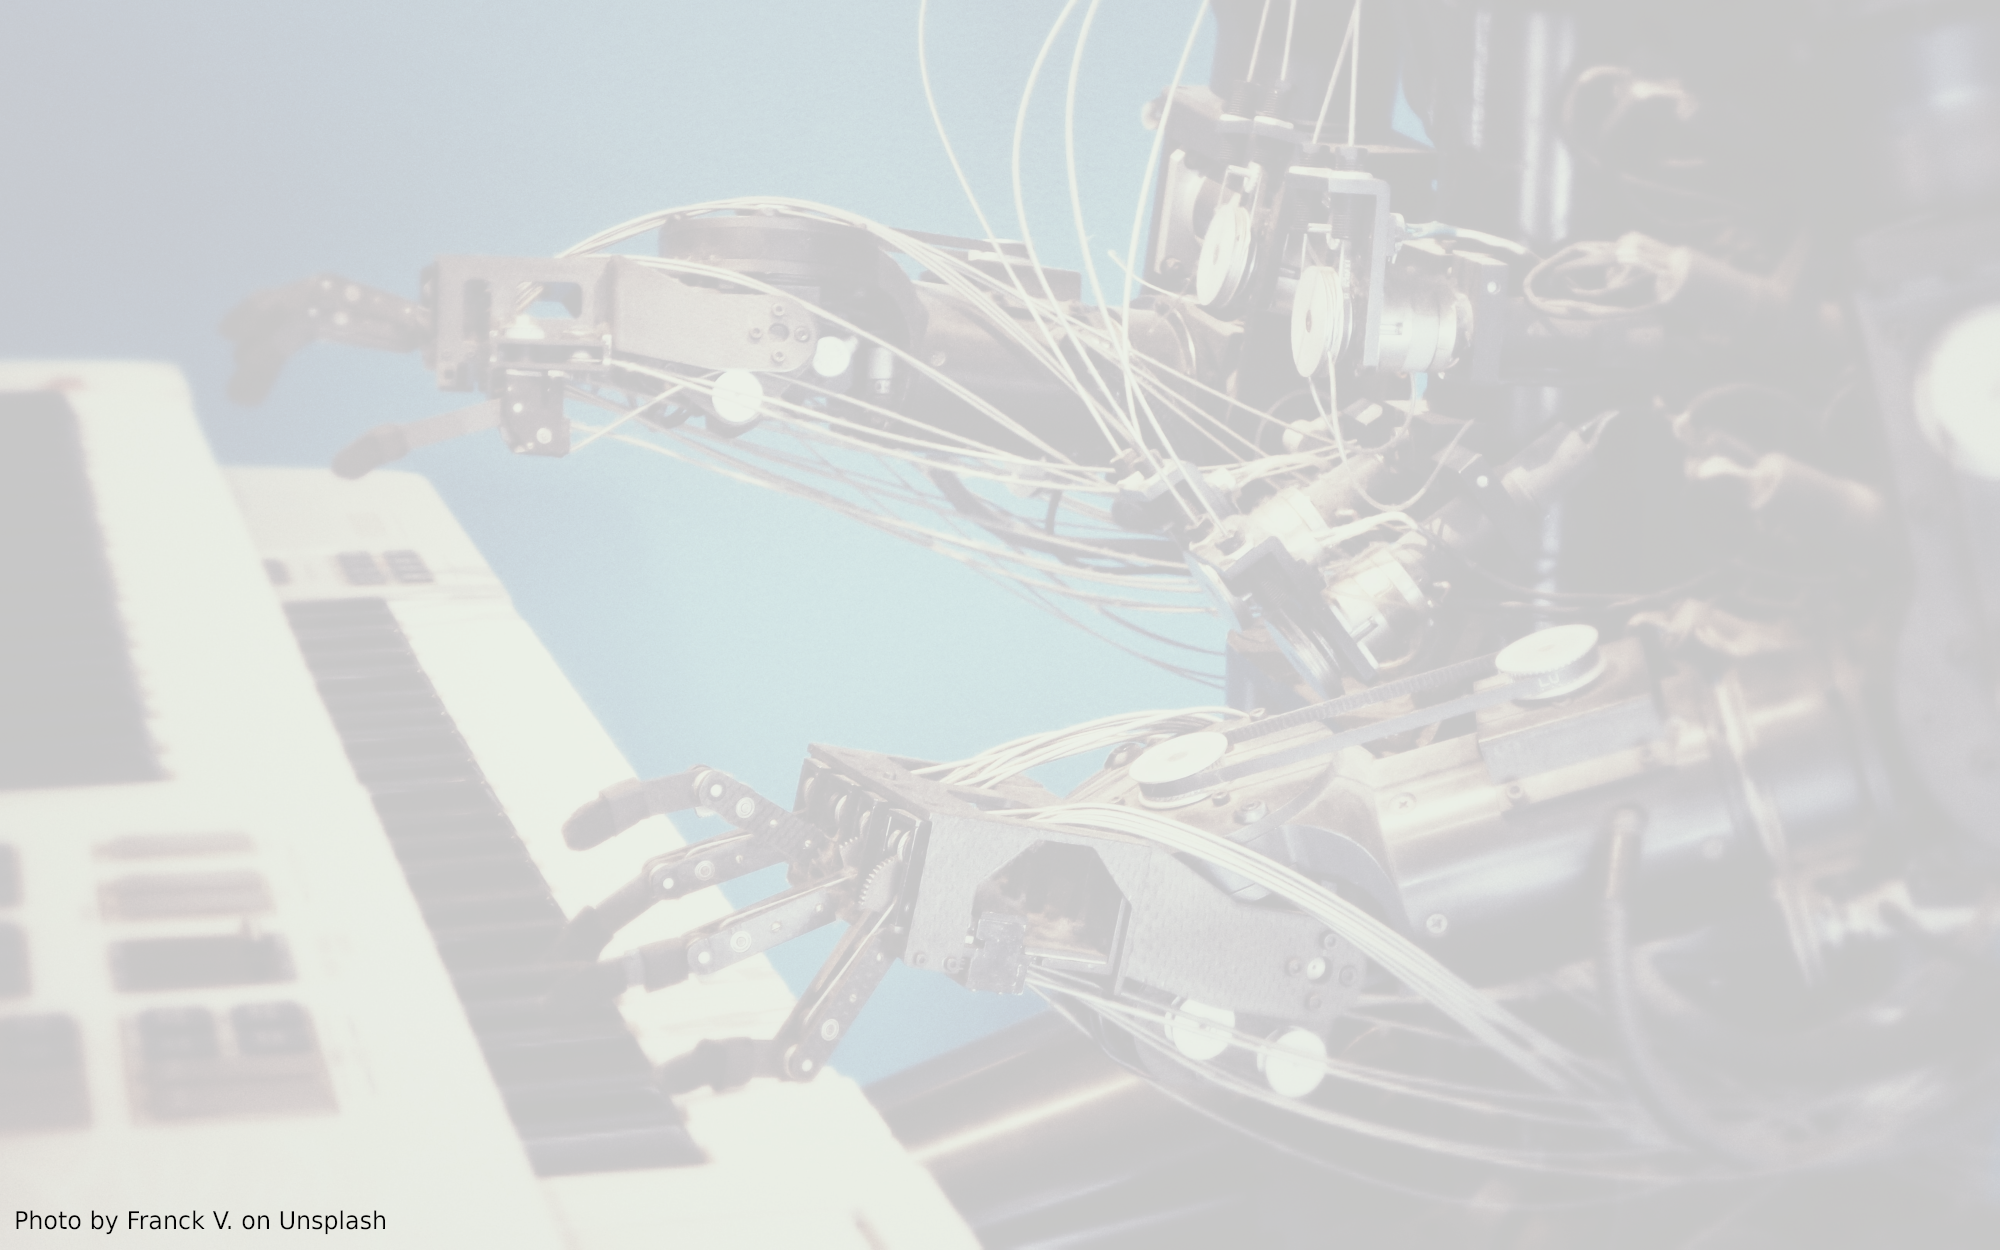
\includegraphics[width=\paperwidth]{figures/franck-v-U3sOwViXhkY-unsplash.png}
}%
\begin{frame}{Optimising for human attention}


\textbf{Humans to figure out what -- computers to do over and over again.}

\begin{itemize}
    \item Changing journals to submit to should not take a week of re-typesetting!
    \item Graphs should automatically generate on changes to data! 
    \item Data should only need to be entered once!
\end{itemize}




\textbf{FAIR and Reproducible Research}

\begin{itemize}
    \item \textit{Excel delinda est!} Let us code our analyses in a testable way! \parencite{Krugman2013-ju, Ross2020-yg, Bruford2020-tw}
    \item Directly and specifically reward data reuse.
    \item Promote reproducing studies as a valid MRes option. \parencite{Spring2018-kr}
\end{itemize}



\end{frame}}

\setbeamertemplate{footline}{%
%\strut~\texttt{https://github.com/MQ-FOAR705/MQ-FOAR705-Week1}%
\hfill\insertframenumber~/~\inserttotalframenumber\strut~~~
}

\begin{frame}{Optimising for novel capabilities}

\textbf{New practices + new knowledge + new tools }
\begin{itemize}
    \item Human + Computer can extend capabilities of both
    \item Technology may make novel research possible -- with an awful lot of blind alleys first.
\end{itemize}

\textbf{Solving the allocation problem is hard}
\begin{itemize}
    \item We need to reward research which might fail.
    \item We need to make failure as cheap, fast, and easy as possible. Reputationally expensive to fail \textit{after} winning the ARC grant.
\end{itemize}

We increase what we reward -- but are the system's rewards aligned to what we say we want? \parencite{Beer2002-tl}
\end{frame}

\section{Illustrative Examples}%

\begin{frame}{Impact: Social Media Research for NSW government}
\begin{columns}[t]
\begin{column}{.35\textwidth}
\textbf{Automated and ethical data collection}
\begin{itemize}
    \item Automated collection: 1.3 million social media posts
    \item Python's Natural Langauge Processing + graphing to collect, process, describe, and visualise data.
\end{itemize}

\end{column}
\begin{column}{.55\textwidth}
\begin{figure}
    \vspace{-.5cm}
    \centering
    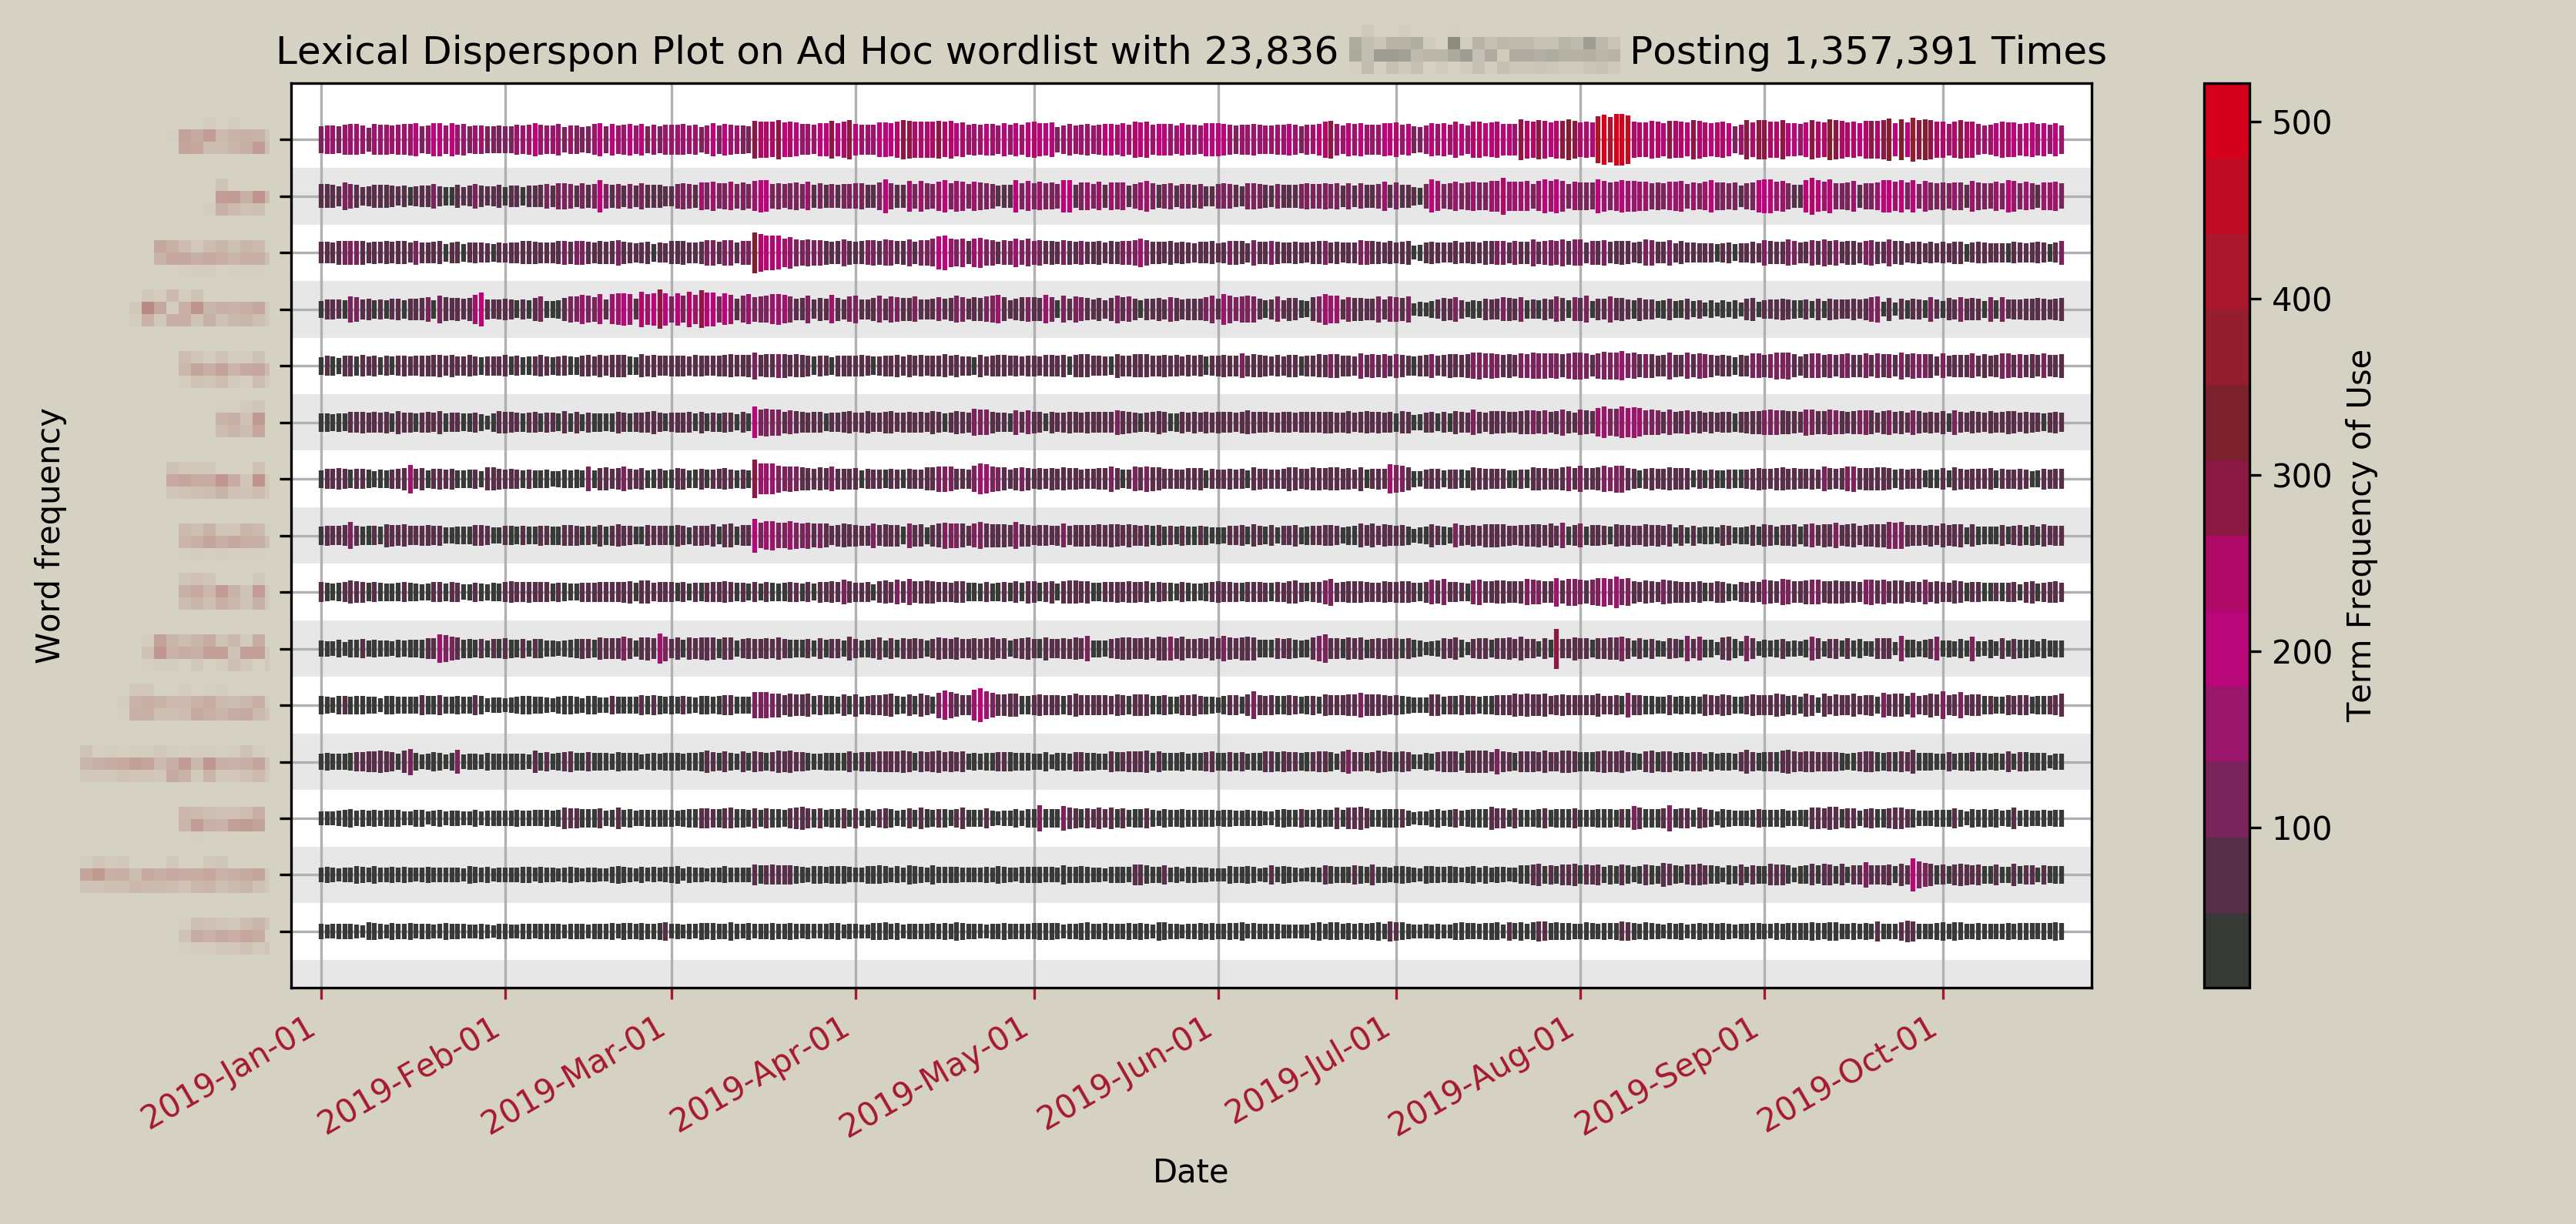
\includegraphics[width=\textwidth]{figures/blur.png}
    \caption{Blurred Lexical Disperson plot from this research}
\end{figure}
\end{column}
\end{columns}
\textbf{High impact}
\begin{itemize}
    \item Policy recommendations backed by thorough and reproducible data. 
    \item Presented to Commonwealth committee this week, state committees in July.
    \item Compliments from the Deputy Minister
    
    
\end{itemize}
\end{frame}

\setbeamertemplate{footline}{%
%\strut~\texttt{https://github.com/MQ-FOAR705/MQ-FOAR705-Week1}%
Fabricius Workbench photo, Apache 2 license\hfill\insertframenumber~/~\inserttotalframenumber\strut~~~
}
{\usebackgroundtemplate{%
\centering

\includegraphics[width=\paperwidth]{figures/fabricius.png}%
}%
\begin{frame}{Engagement: Google Arts and Culture and Fabricius}

\begin{itemize}
    \item \url{artsandculture.google.com/partner/macquarie-university}
    \begin{itemize}
    \item Google Arts and Culture: ` is to preserve and bring the world’s art and culture online so it’s accessible to anyone, anywhere.' \parencite{Google_Arts_and_Culture2020-ga}
    \item 15,820 views from 142 countries on MQ's Arts and Culture pages in July
    \item A link on google.com.au under the search bar on 6 August: `Discover the language of the ancient Egyptians: decode hieroglyphs using AI'
    \end{itemize}
    \item \url{g.co/fabricius}
    \begin{itemize}
    \item Google Cloud Machine Learning + Ancient Egyptian Hieroglyphs
    \item 230 press stories around world
    \item Approving tweet to us from Australian ambassador to Egypt
    \item We have top billing as partner
    \item Cute extra items to engage social media and encourage kids to learn.
    \end{itemize}
\end{itemize}

\end{frame}}
\setbeamertemplate{footline}{%
%\strut~\texttt{https://github.com/MQ-FOAR705/MQ-FOAR705-Week1}%
\hfill\insertframenumber~/~\inserttotalframenumber\strut~~~
}

\section{Macquarie's Strategic Transformation}

\begin{frame}{Advocacy and Advice}
\textbf{Focused investment in Research result: `Improved access to, and quality of, shared research facilities and infrastructure with a focus on providing institution-level facilities'}

\begin{itemize}
    \item We find establishing tools hard
    \item Persuading joyful adoption is harder -- hard to fake a value proposition except through threat of punishment
\end{itemize}

\textbf{Digital Transformation measure: `Adoption of new technology and ways of working.'}
\begin{itemize}
    \item Being a \textit{useful} advocate to solve \textit{specific problems}
    \item Demonstrate that new systems promise higher reward relative to increased risk
\end{itemize}
\end{frame}

\begin{frame}{Capability-building and Compliance}

\textbf{Focused investment in Research result: `Improved upon the results of ERA and EI 2018'}

\begin{itemize}
    \item Reduce exposure to data breaches,  scandals, and disruptions to research continuity through data-loss.
    \item Increase technical options for high engagement and opportunities for impact.
    \item Show people how to reduce frustration with proper typesetting and citation management.
\end{itemize}
\end{frame}

\begin{frame}{Capability-building and Compliance}
\textbf{Ways of Working measure: `Staff engagement and retention, specifically in career development'}
\begin{itemize}
    \item The Carpentries is \textit{only a start}. It is necessary but not sufficient.
    \item Showing faculty and staff how to solve \textit{small} problems with code creates a community and a foundation.
    \item Guide researchers into considering what tools to learn and use, rather than reaching for comfortable, slow, default.
\end{itemize}
\end{frame}


% \begin{frame}{Guiding results and measures}
% Relevant operating plan items: 
% \begin{itemize}
%     \item Focused investment in Research result: `Improved upon the results of ERA and EI 2018'
%     \item Focused investment in Research result: `Improved access to, and quality of, shared research facilities and infrastructure with a focus on providing institution-level facilities'
%     \item Ways of Working measure: `Staff engagement and retention, specifically in career development'
%     \item Digital Transformation measure: `Adoption of new technology and ways of working.'
% \end{itemize}

% Caution via `Goodhart's Law': `When a measure becomes a target, it ceases to be a good measure.'

% \end{frame}

% \begin{frame}{Research Quality, Engagement and Impact}
% \end{frame}

% \begin{frame}{Infrastructure use and access}
% \end{frame}

% \begin{frame}{Career development}
% \end{frame}

% \begin{frame}{Adoption of new technology}
% \end{frame}
% Emergent technologies are assessed and deployed where they add value to education, research, student and engagement
% Digital skills and capabilities of education and research staff drive the successful transition to digital platforms



\section{Issues for consideration}
\begin{frame}{Many strategic issues}
\textbf{Valuing researcher/staff time,  risk-taking, and building general capability}
\begin{itemize}
    \item How do we create space for staff to risk their time on novel techniques?
    \item How do we treat researcher and staff time-value versus money?
    \item How do we get our system to reward general skill/capability building?
\end{itemize}
    
\textbf{Pay attention to university feedback and reward loops}    
    \begin{itemize}
    \item What, specifically, do we reward -- and does it support better data practices?
    \item What are our feedback loops? How long to learn about failure?
\end{itemize}


Caution via `Goodhart's Law': 'When a measure becomes a target, it ceases to be a good measure.` \parencite{Strathern1997-du, Goodhart1975-cq}

\end{frame}



\begin{frame}{Thank you!}

% This presentation is available at:
% \texttt{https://osf.io/...}

A citable resource containing \LaTeX{} source code and this compiled presentation is available at: \url{https://osf.io/y5c7n/}

This work is licensed CC-BY-SA 4.0 International, by: Brian Ballsun-Stanton. 

\end{frame}


\setbeamertemplate{footline}{%
%\strut~\texttt{https://github.com/MQ-FOAR705/MQ-FOAR705-Week1}%

}

\begin{frame}[allowframebreaks, noframenumbering]{References}
%\begin{multicols*}{2}
%\raggedcolumns
\printbibliography[heading=none]
%\end{multicols*}
\end{frame}





\end{document}